




%%
\documentclass[1p,12pt]{elsarticle}\usepackage[]{graphicx}\usepackage[]{color}
%% maxwidth is the original width if it is less than linewidth
%% otherwise use linewidth (to make sure the graphics do not exceed the margin)
\makeatletter
\def\maxwidth{ %
  \ifdim\Gin@nat@width>\linewidth
    \linewidth
  \else
    \Gin@nat@width
  \fi
}
\makeatother

\definecolor{fgcolor}{rgb}{0.345, 0.345, 0.345}
\newcommand{\hlnum}[1]{\textcolor[rgb]{0.686,0.059,0.569}{#1}}%
\newcommand{\hlstr}[1]{\textcolor[rgb]{0.192,0.494,0.8}{#1}}%
\newcommand{\hlcom}[1]{\textcolor[rgb]{0.678,0.584,0.686}{\textit{#1}}}%
\newcommand{\hlopt}[1]{\textcolor[rgb]{0,0,0}{#1}}%
\newcommand{\hlstd}[1]{\textcolor[rgb]{0.345,0.345,0.345}{#1}}%
\newcommand{\hlkwa}[1]{\textcolor[rgb]{0.161,0.373,0.58}{\textbf{#1}}}%
\newcommand{\hlkwb}[1]{\textcolor[rgb]{0.69,0.353,0.396}{#1}}%
\newcommand{\hlkwc}[1]{\textcolor[rgb]{0.333,0.667,0.333}{#1}}%
\newcommand{\hlkwd}[1]{\textcolor[rgb]{0.737,0.353,0.396}{\textbf{#1}}}%
\let\hlipl\hlkwb

\usepackage{framed}
\makeatletter
\newenvironment{kframe}{%
 \def\at@end@of@kframe{}%
 \ifinner\ifhmode%
  \def\at@end@of@kframe{\end{minipage}}%
  \begin{minipage}{\columnwidth}%
 \fi\fi%
 \def\FrameCommand##1{\hskip\@totalleftmargin \hskip-\fboxsep
 \colorbox{shadecolor}{##1}\hskip-\fboxsep
     % There is no \\@totalrightmargin, so:
     \hskip-\linewidth \hskip-\@totalleftmargin \hskip\columnwidth}%
 \MakeFramed {\advance\hsize-\width
   \@totalleftmargin\z@ \linewidth\hsize
   \@setminipage}}%
 {\par\unskip\endMakeFramed%
 \at@end@of@kframe}
\makeatother

\definecolor{shadecolor}{rgb}{.97, .97, .97}
\definecolor{messagecolor}{rgb}{0, 0, 0}
\definecolor{warningcolor}{rgb}{1, 0, 1}
\definecolor{errorcolor}{rgb}{1, 0, 0}
\newenvironment{knitrout}{}{} % an empty environment to be redefined in TeX

\usepackage{alltt}

%% Use the option review to obtain double line spacing


%% The graphicx package provides the includegraphics command.
\usepackage{graphicx}
%% The amssymb package provides various useful mathematical symbols
\usepackage{amssymb}

\usepackage{lineno}



% \biboptions{}
\IfFileExists{upquote.sty}{\usepackage{upquote}}{}
\begin{document}

\begin{frontmatter}

%% Title, authors and addresses

\title{Pea Plants and Diet Coke: An Experiment}

\author{Jacob Dym and Paul Harmon}

\address{Montana State University}

\begin{abstract}
%% Text of abstract
In order to assess the effects of Diet Coke on the short term growth behavior of plants, we grew pea plants and treated them with different combinations of watering type and plant food. Alaska pea plants were grown in cups treated with a watering regimen consisting of either Diet Coke, diluted Diet Coke, or water. They were also randomized to a combination of either getting plant food upon being planted or not receiving any. A mixed-model was fit to analyze the fixed effects of the two factors while accounting for differences in variation due to the cups and row-blocks in the Randomized block design. Results indicate that pea plants treated with some form of diet coke grew taller than those that were treated with water, regardless of whether or not they received plant food. 
\end{abstract}


\end{frontmatter}

%%
%% Start line numbering here if you want
%%


%% main text
\section{Introduction and Research Questions}

The effect of aspartame, sodium, and other chemical consumption on health outcomes of diet soft-drink consumers has motivated many recent academic studies and garnered attention in the mainstream media. Diet Coke (as well as other brands of diet soda) has been shown to be associated with changes in metabolic behavior and other physiological responses (Veldhuizen, 2017). It has also been linked in longitudinal observational studies to increased risk of stroke. Perhaps unsurprisingly, according to survey analysis performed by Nielsen, diet soda consumption is on the decline, perhaps due to the growing perception that Diet Coke simply is not a healthy choice . But is Diet Coke that bad for consumers? After all, Diet Coke is mostly water (Levitt, 2007). Most scientific work focuses on long-term impacts of soft drink consumption on health via longitudinal studies; however, very little dedicated experimentation has been done to test either its short or long term effects on either humans or plant life. 

The purpose of our experiment, then, is to analyze the short-term effects of Diet Coke on plant growth when used as a substitute for water. The research question addressed by this study is as follows: Does Diet Coke harm the ability of a plant to grow? We posit that since Diet Coke contains ingredients that may be harmful, including aspartame, plants treated exclusively with it instead of water will grow at
a diminished rate relative to those treated with actual water. Based on this, the treatment of interest is whether the plant is watered with pure tap water or a mixture involving Diet Coke. The treatments of this factor are:

\begin{itemize}
\item Diet Coke
\item 22 percent Diet Coke Dilution
\item Tap water (Control)
\end{itemize}

We are also interested in the effect of plant food,  especially whether or not the effect of Diet Coke is modified by the presence or absence of plant food.  It seems possible that the Diet Coke could react differently with soil enriched with plant food than in would with soil that was not enriched at all. 

\begin{itemize}
\item Plant Food (administered at planting)
\item No plant food
\end{itemize}

Previous research has been done on the effect of different types of watering substances on pea plant growth. Work done by Roland et al (2013) found significant differences in pea plant heights when comparing Vitamin Water treatments to an untreated watering regime. Similarly, work by Slutzky et al (2003) found significant differences between pea-plant heights after treatment with unspecified Diet soda, Water, ibuprofen, and sparkling water regimes. However, little appears to have been done to specifically assess the effect of Diet Coke specifically, nor has there been much progress on the assessment of an interaction between presence of plant food and watering type.   



\section{Methods}
\subsection{Experimental Design}

The experiment was set up so that 4 pea plants were grown together in cups. This way, we avoided cross contamination of watering treatments because all plants within a single cup received the same treatement.  In order to discourage pea roots from growing into each other, peas were planted at each of the cardinal directios in the cups as denoted in Figure X. 
 \begin{figure}[h!]
 	\caption{Blocking arrangement of the peas}
 	\centering
	
\includegraphics[width = 7cm]{pea_locations.png}
\end{figure}


6 cups were arranged in row-blocks in a cardboard box that was placed on a table next to a west-facing window. The plants received between 5 and 7 hours of sunlight daily.  Peas were watered once daily in the evening; each treatment consisted of between 20 and 25 ml of either Diet Coke, diluted Diet Coke, or tap water. Per instructions, plant food was administered at planting only via addition to and mixing in the soil.  

Figure X shows the experimental design. Treatments (imposed to each cup) were randomized within each block and up to four pea plants could germinate within a single cup. Ideally, this would have led to 96 pea plants; however, some did not germinate. This is discussed further in the germination section of this paper. 

 \begin{figure}[h!]
 	\caption{Blocking arrangement of the peas}
 	\centering
	
\includegraphics[width = 7cm]{figure/blocking_arrangment.png}
\end{figure}


Figure X shows the setup of the experiment at planting. Pea plants were subject to between 5 and 7 hours of sunlight per day; however it is possible that plants nearer the window could have received more intense sunlight than those farther from the window. This was the reason for consideration of row-blocks. This experiment utilized Jiffy brand plant starting mix for soil, Expert plant food, and Ferry-Morse alaska pea seeds, all purchased from the Bozeman Wal Mart. 

 \begin{figure}[h!]
 	\caption{Setup of the initial experiment}
 	\centering
	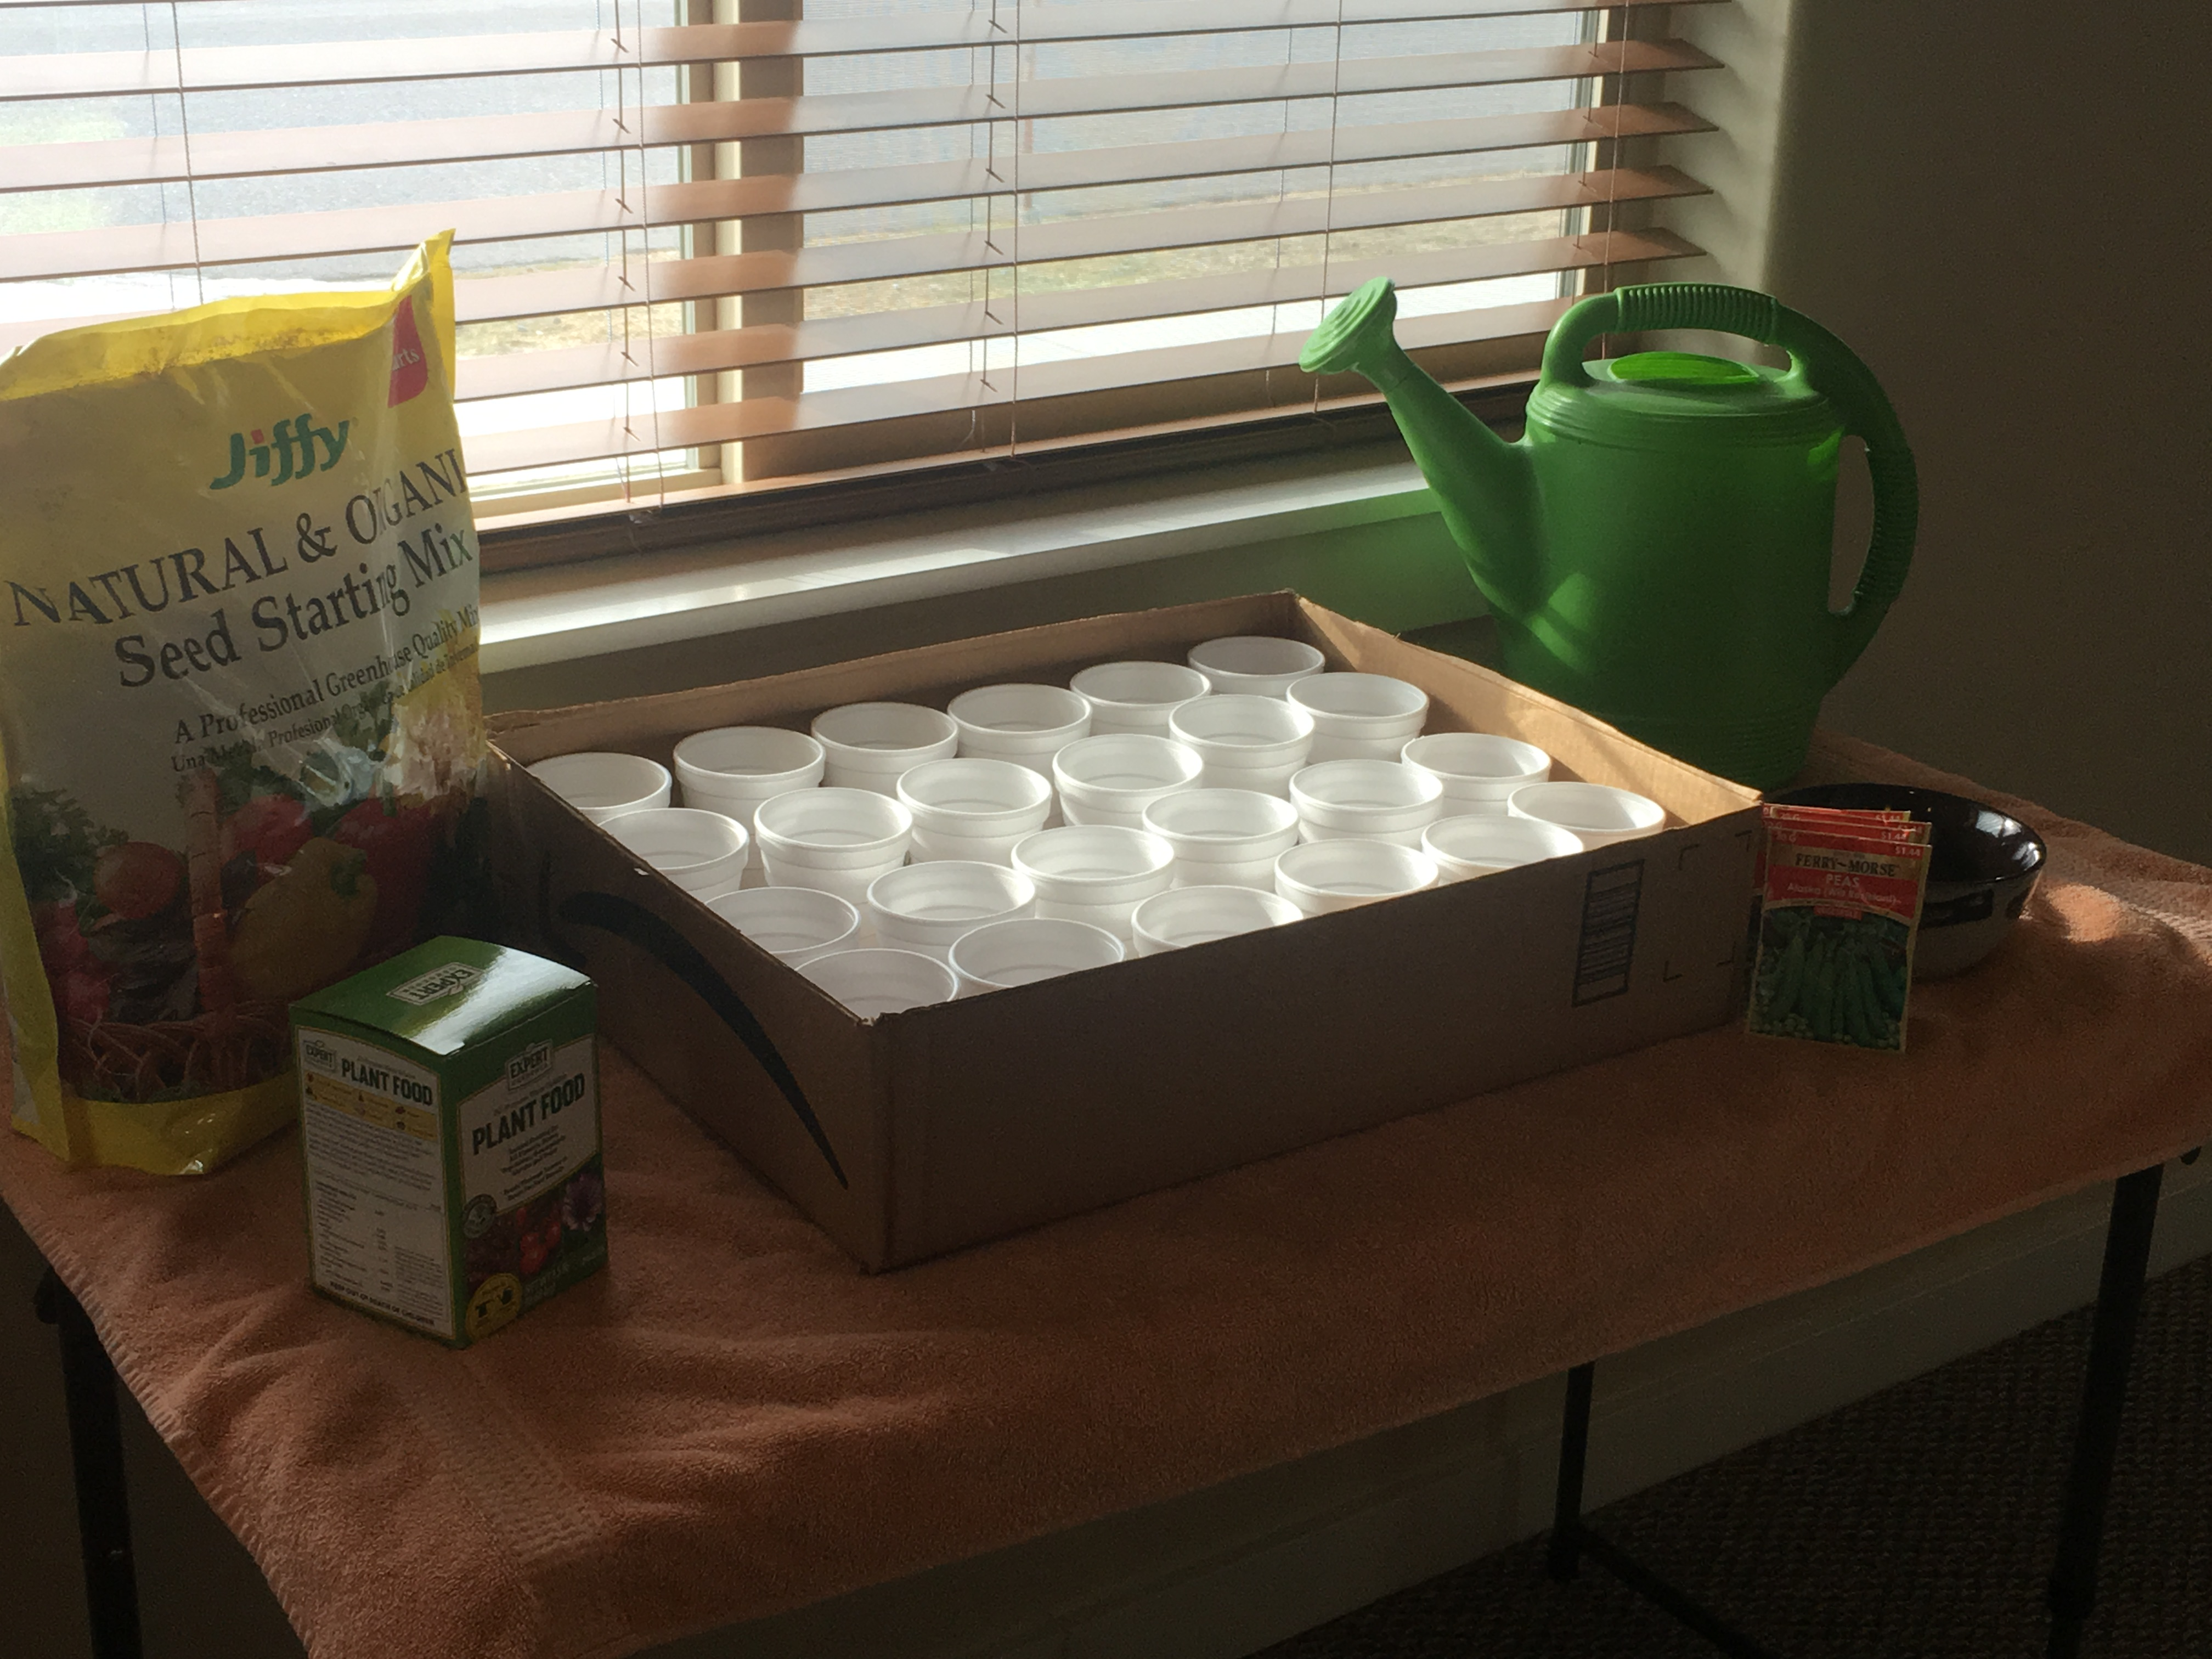
\includegraphics[width = 7cm]{figure/setup.JPG}
\end{figure}

Prior to the start of the study, power calculations were run using values obtained from previous research.  We based our calculations on a simulation study in which true treatment effects were estimated to be 5 mm between each of the treatment groups. Based on the study, in the presence of little block-to-block and cup-to-cup variability, we needed at least 2 replications per treatment, which we greatly exceeded in the actual study. 


\subsection{Data}

\subsection{Statistical Model}
In order to analyze these data, we proposed an analysis that considers the effects of the covariates, as well as the block and cup effects modeled as random effects. Thus our proposed model is: 
\\
\begin{equation}
Y_{ijkl} = \mu + \alpha_i + \beta_j + Block_j + \alpha\beta_{ij}+ Cup_{kj} + \epsilon_{ijkl}
\end{equation}
\\
In the model, the response Y refers to the mean height, in millimeters, of the lth pea plant in the kth cup in the jth block. The overall mean height is $\mu$, the effect of Diet Coke type is $\alpha$, and the effect of fertilizer is $\beta$. We also consider their interaction. The random effects of Cup and Block are also considered in the model, and we make the assumptions that independent random errors are distributed as such: $\epsilon \sim N(0,\sigma^2_{error})$, $Block \sim N(0,\sigma^2_{block})$, and $Cup \sim N(0,\sigma^2_{cup})$. 





\section{Results and Analysis}
\subsection{Experiment Results}

The experiment started on March 21, when plants were initially planted. A 24 hour regularization period occurred before the treatments were imposed. Watering regimes were imposed for the two week period before plant heights were measured on April 5th. Figure X shows the original experimental set up. Figure X shows the plant growth after a week, and then finally Figure X shows the plant growth after the two week period of treatment.  On the whole, the plants responeded well to the treatments; plants grew more than anticipated during the study period. 
 \begin{figure}[h!]
 	\caption{Pea plants at planting, after one week, and at experiment end}
 	\centering
	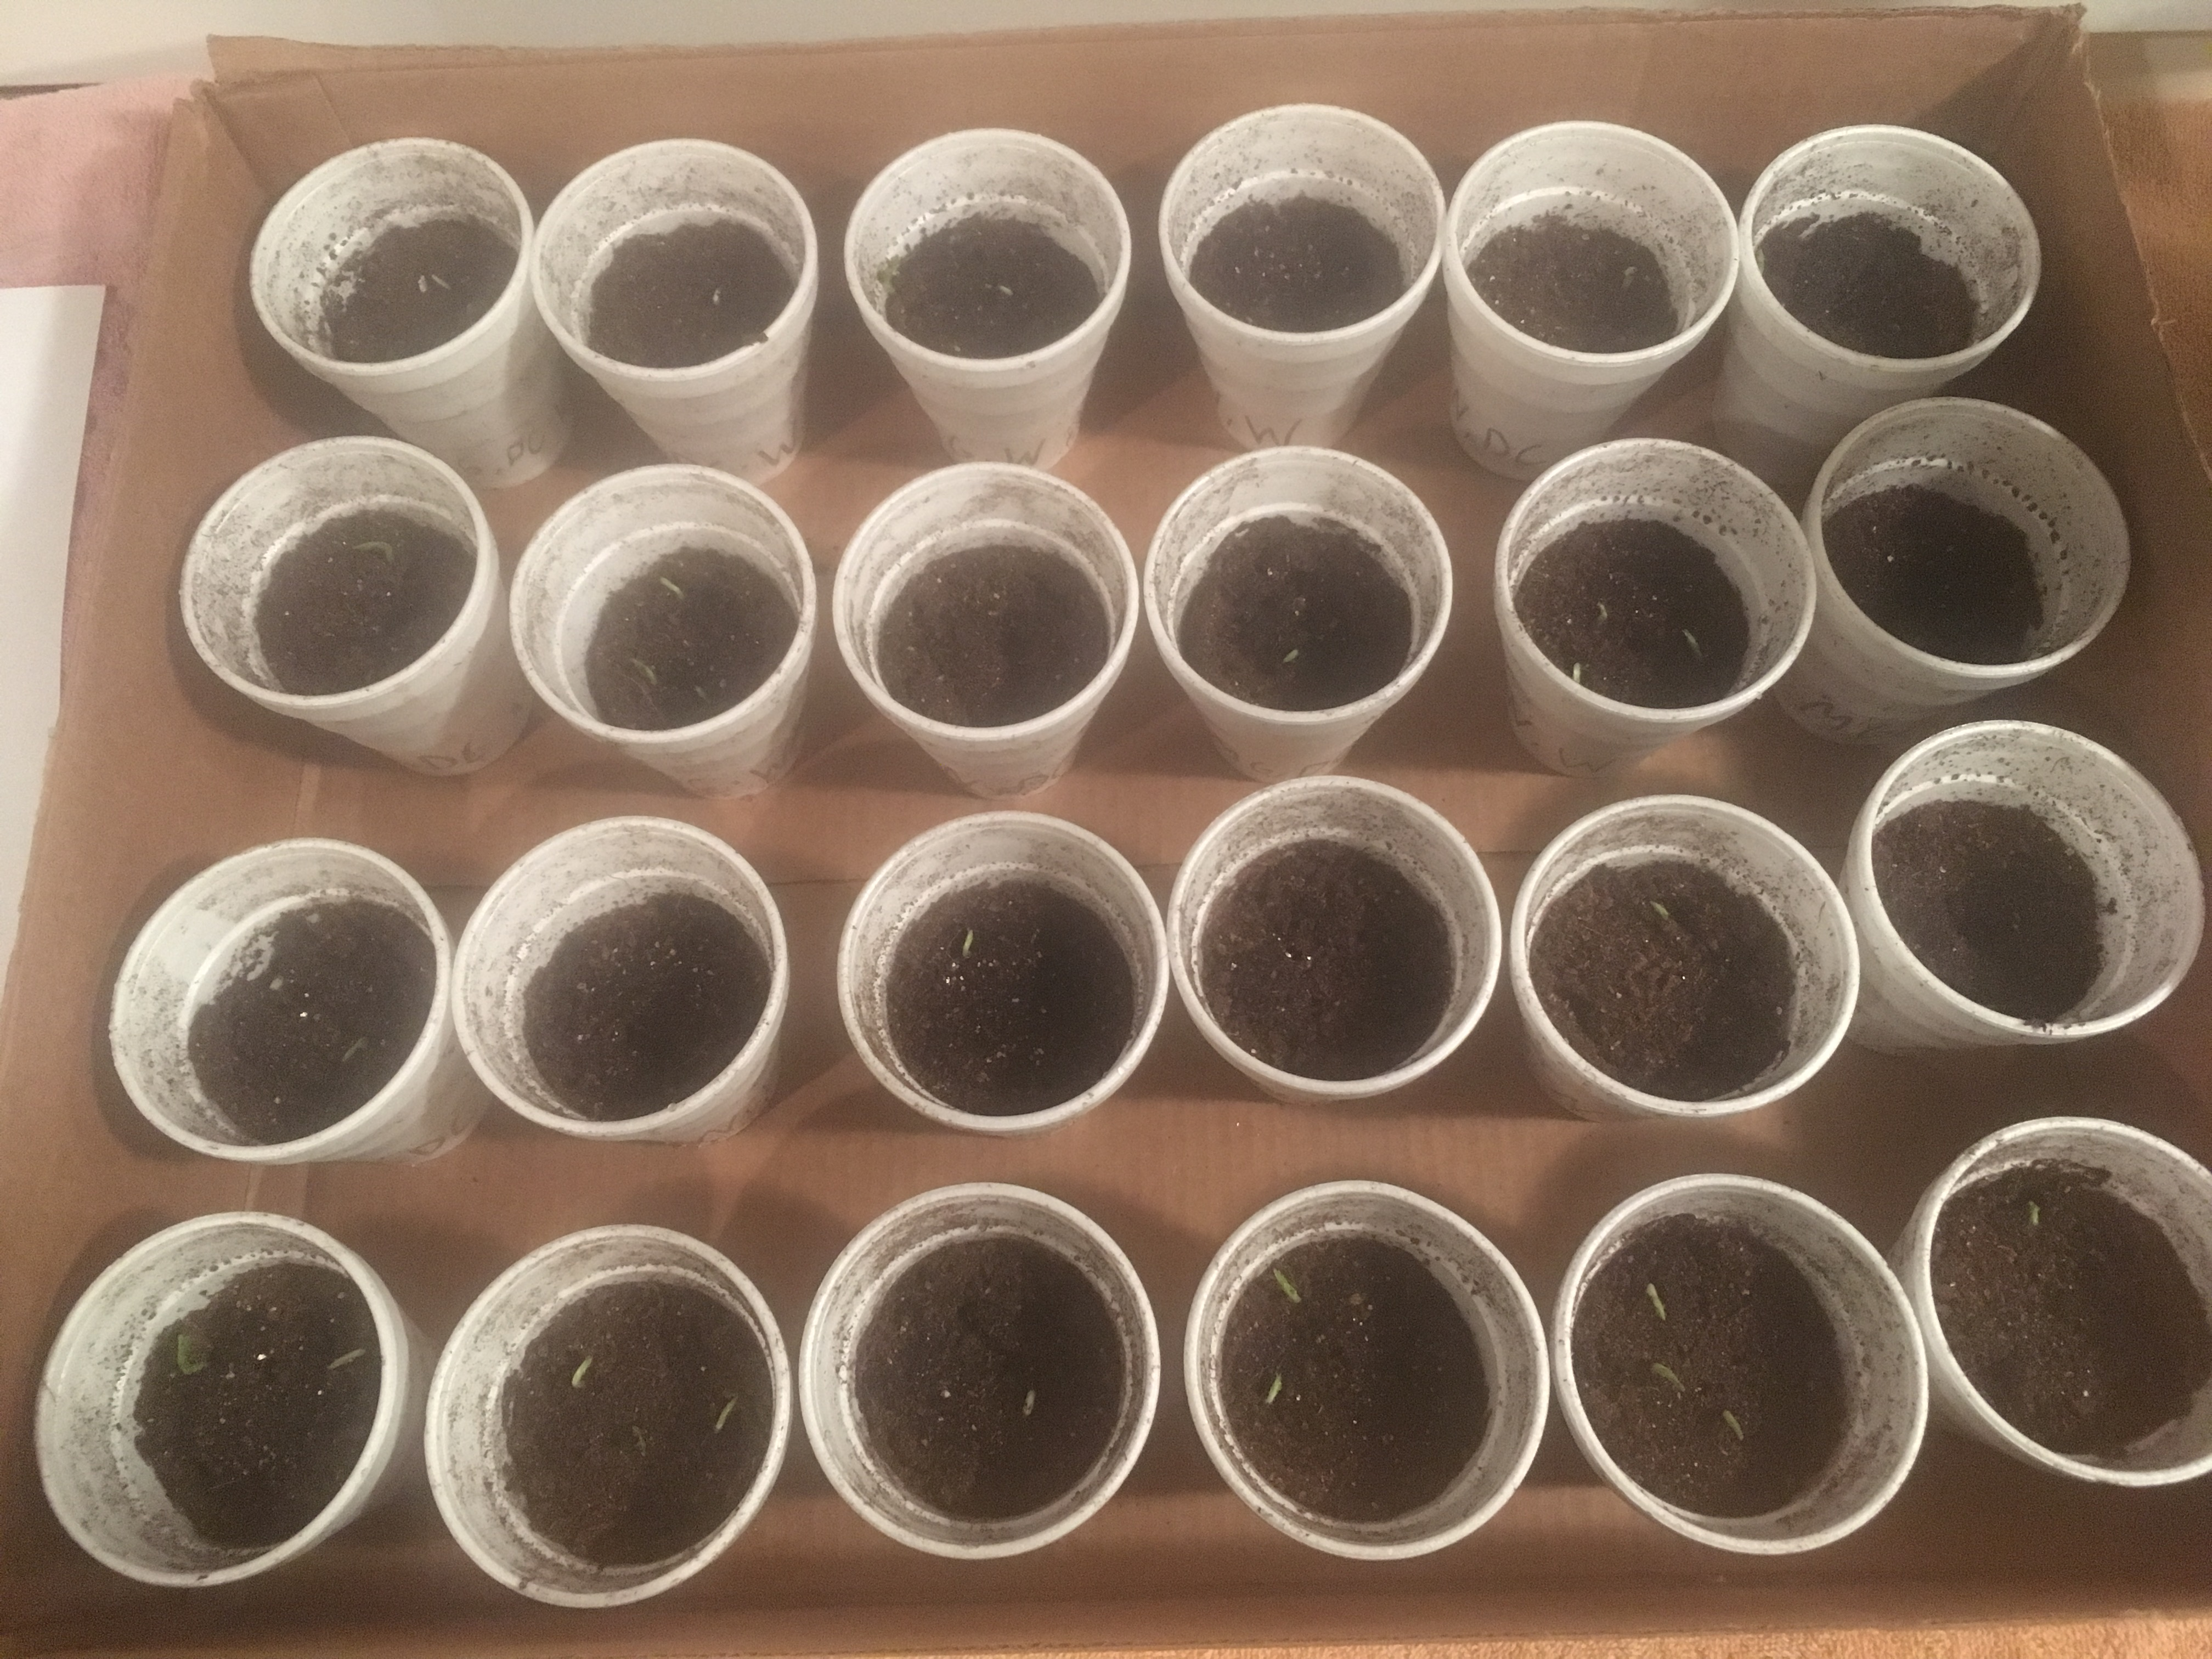
\includegraphics[width = 4cm]{figure/initial_growth.JPG}
	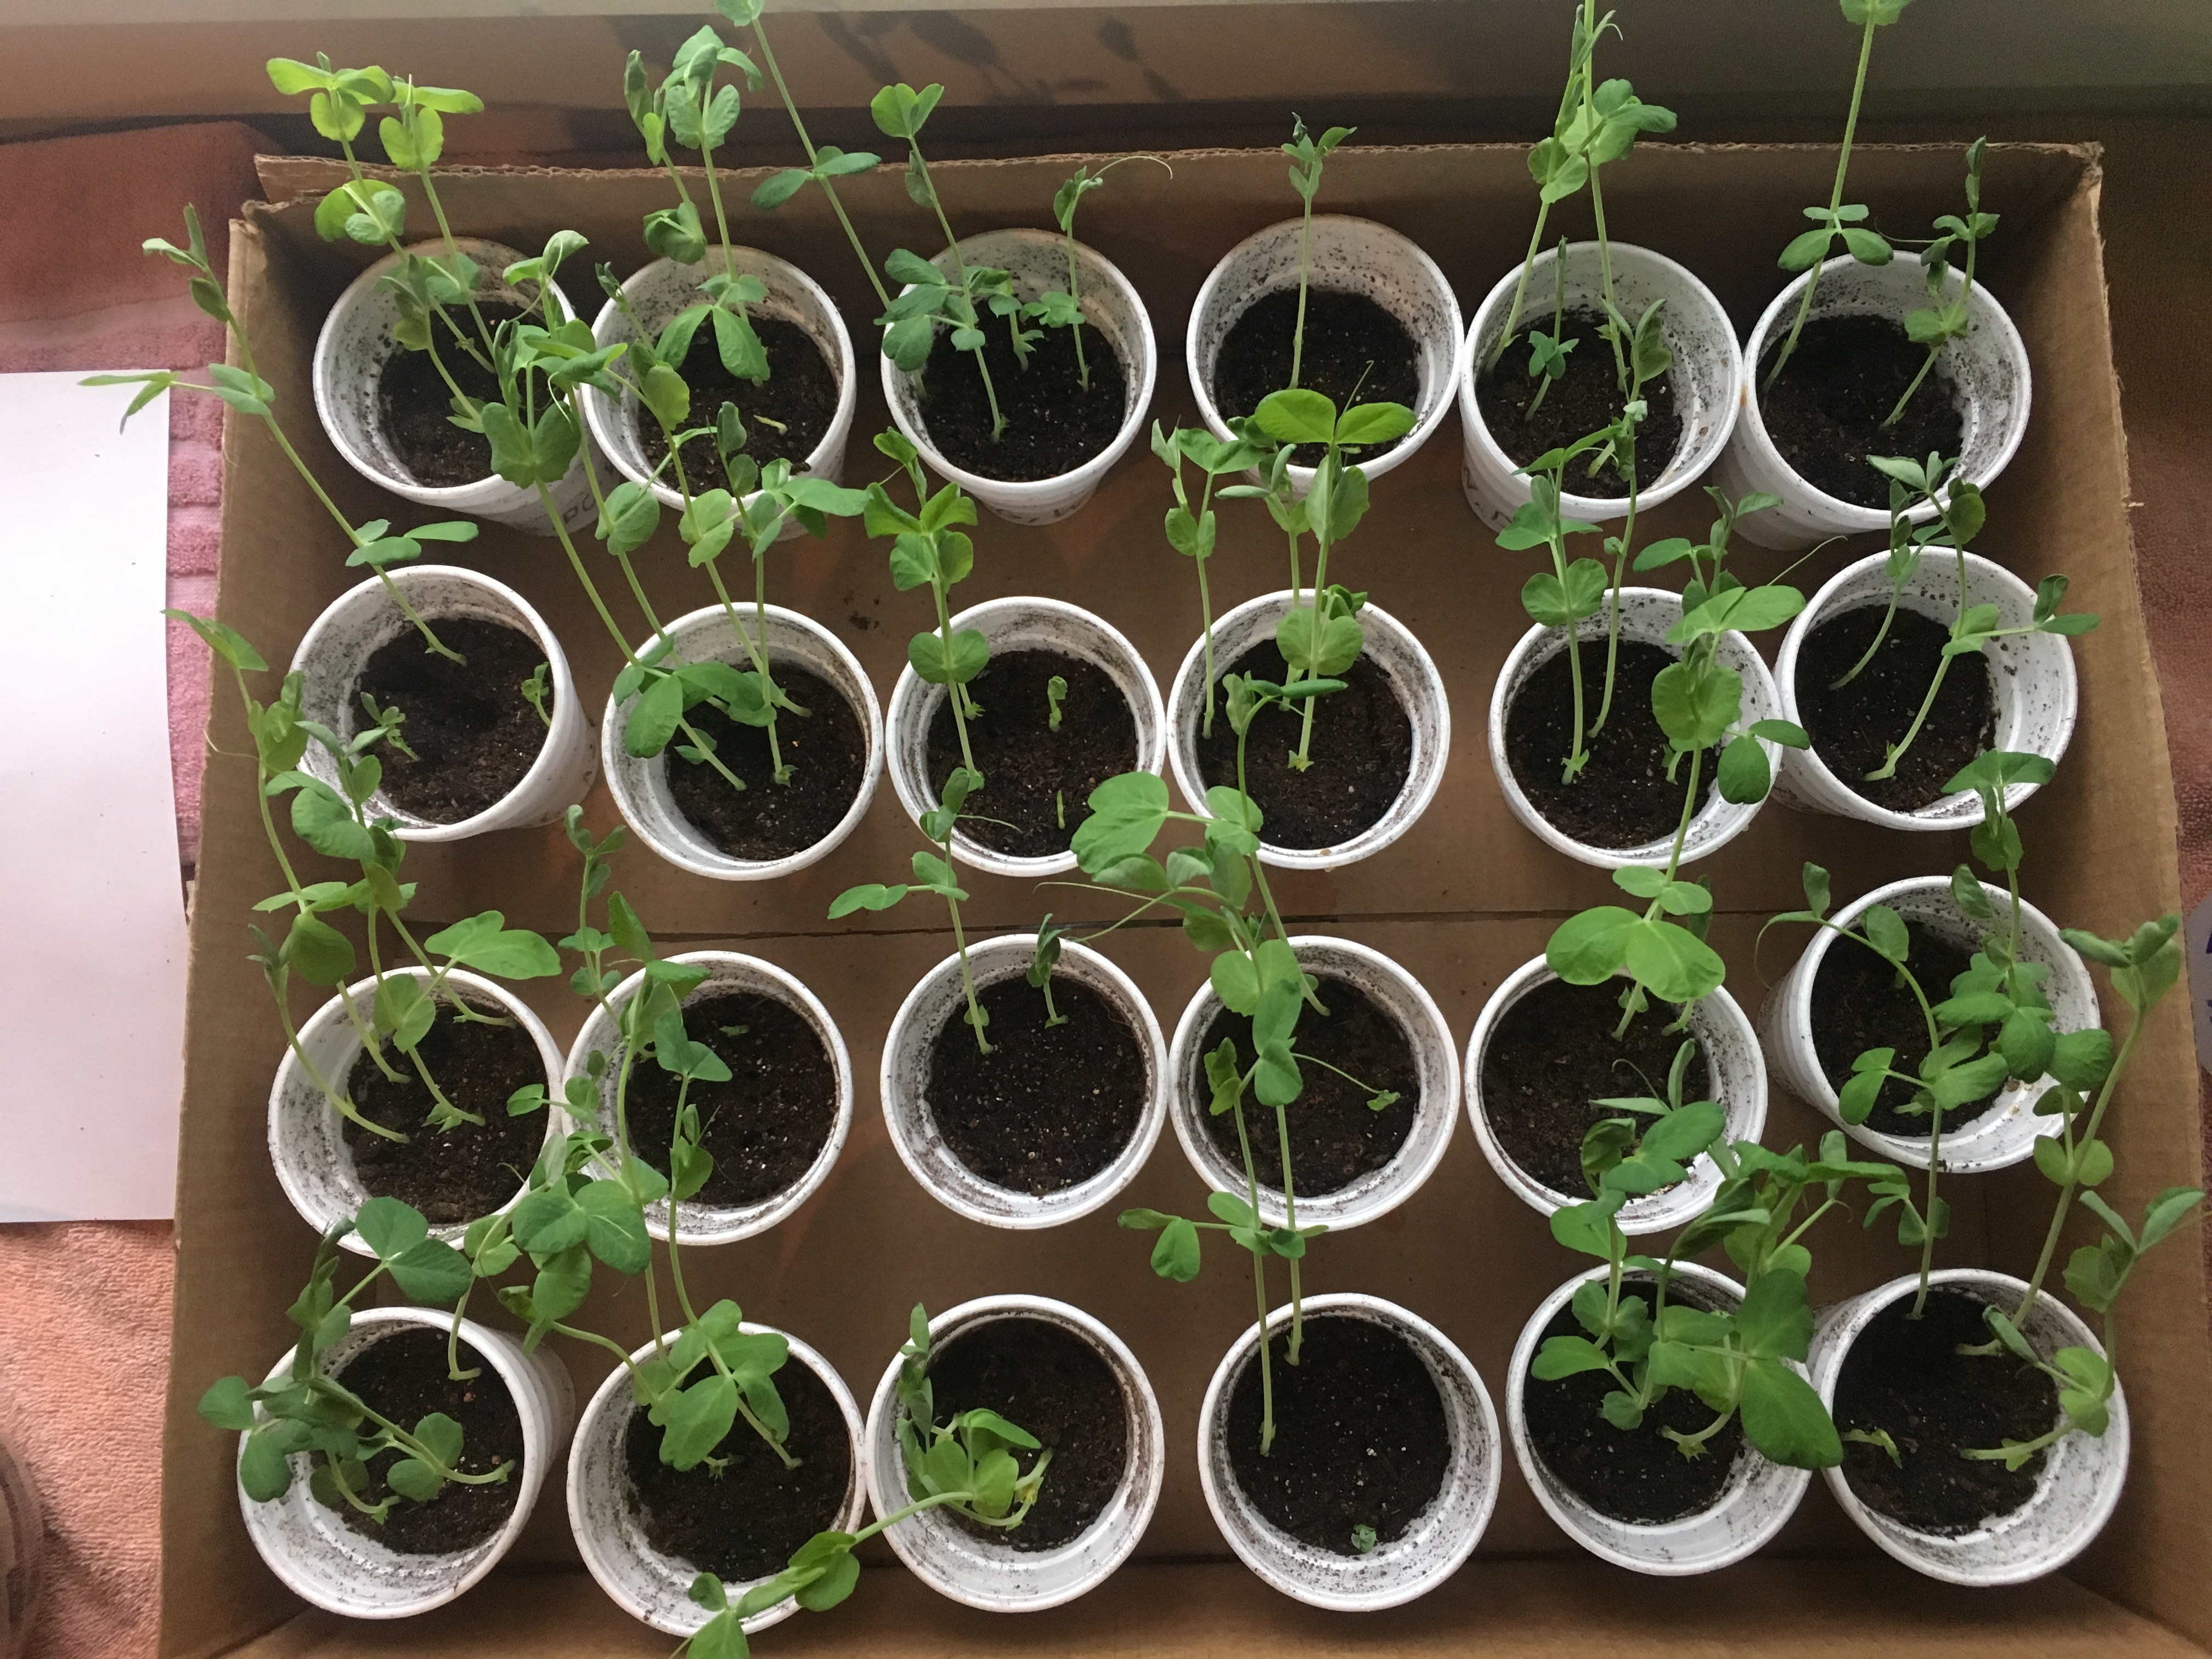
\includegraphics[width = 4cm]{figure/lategrowth.JPG}
	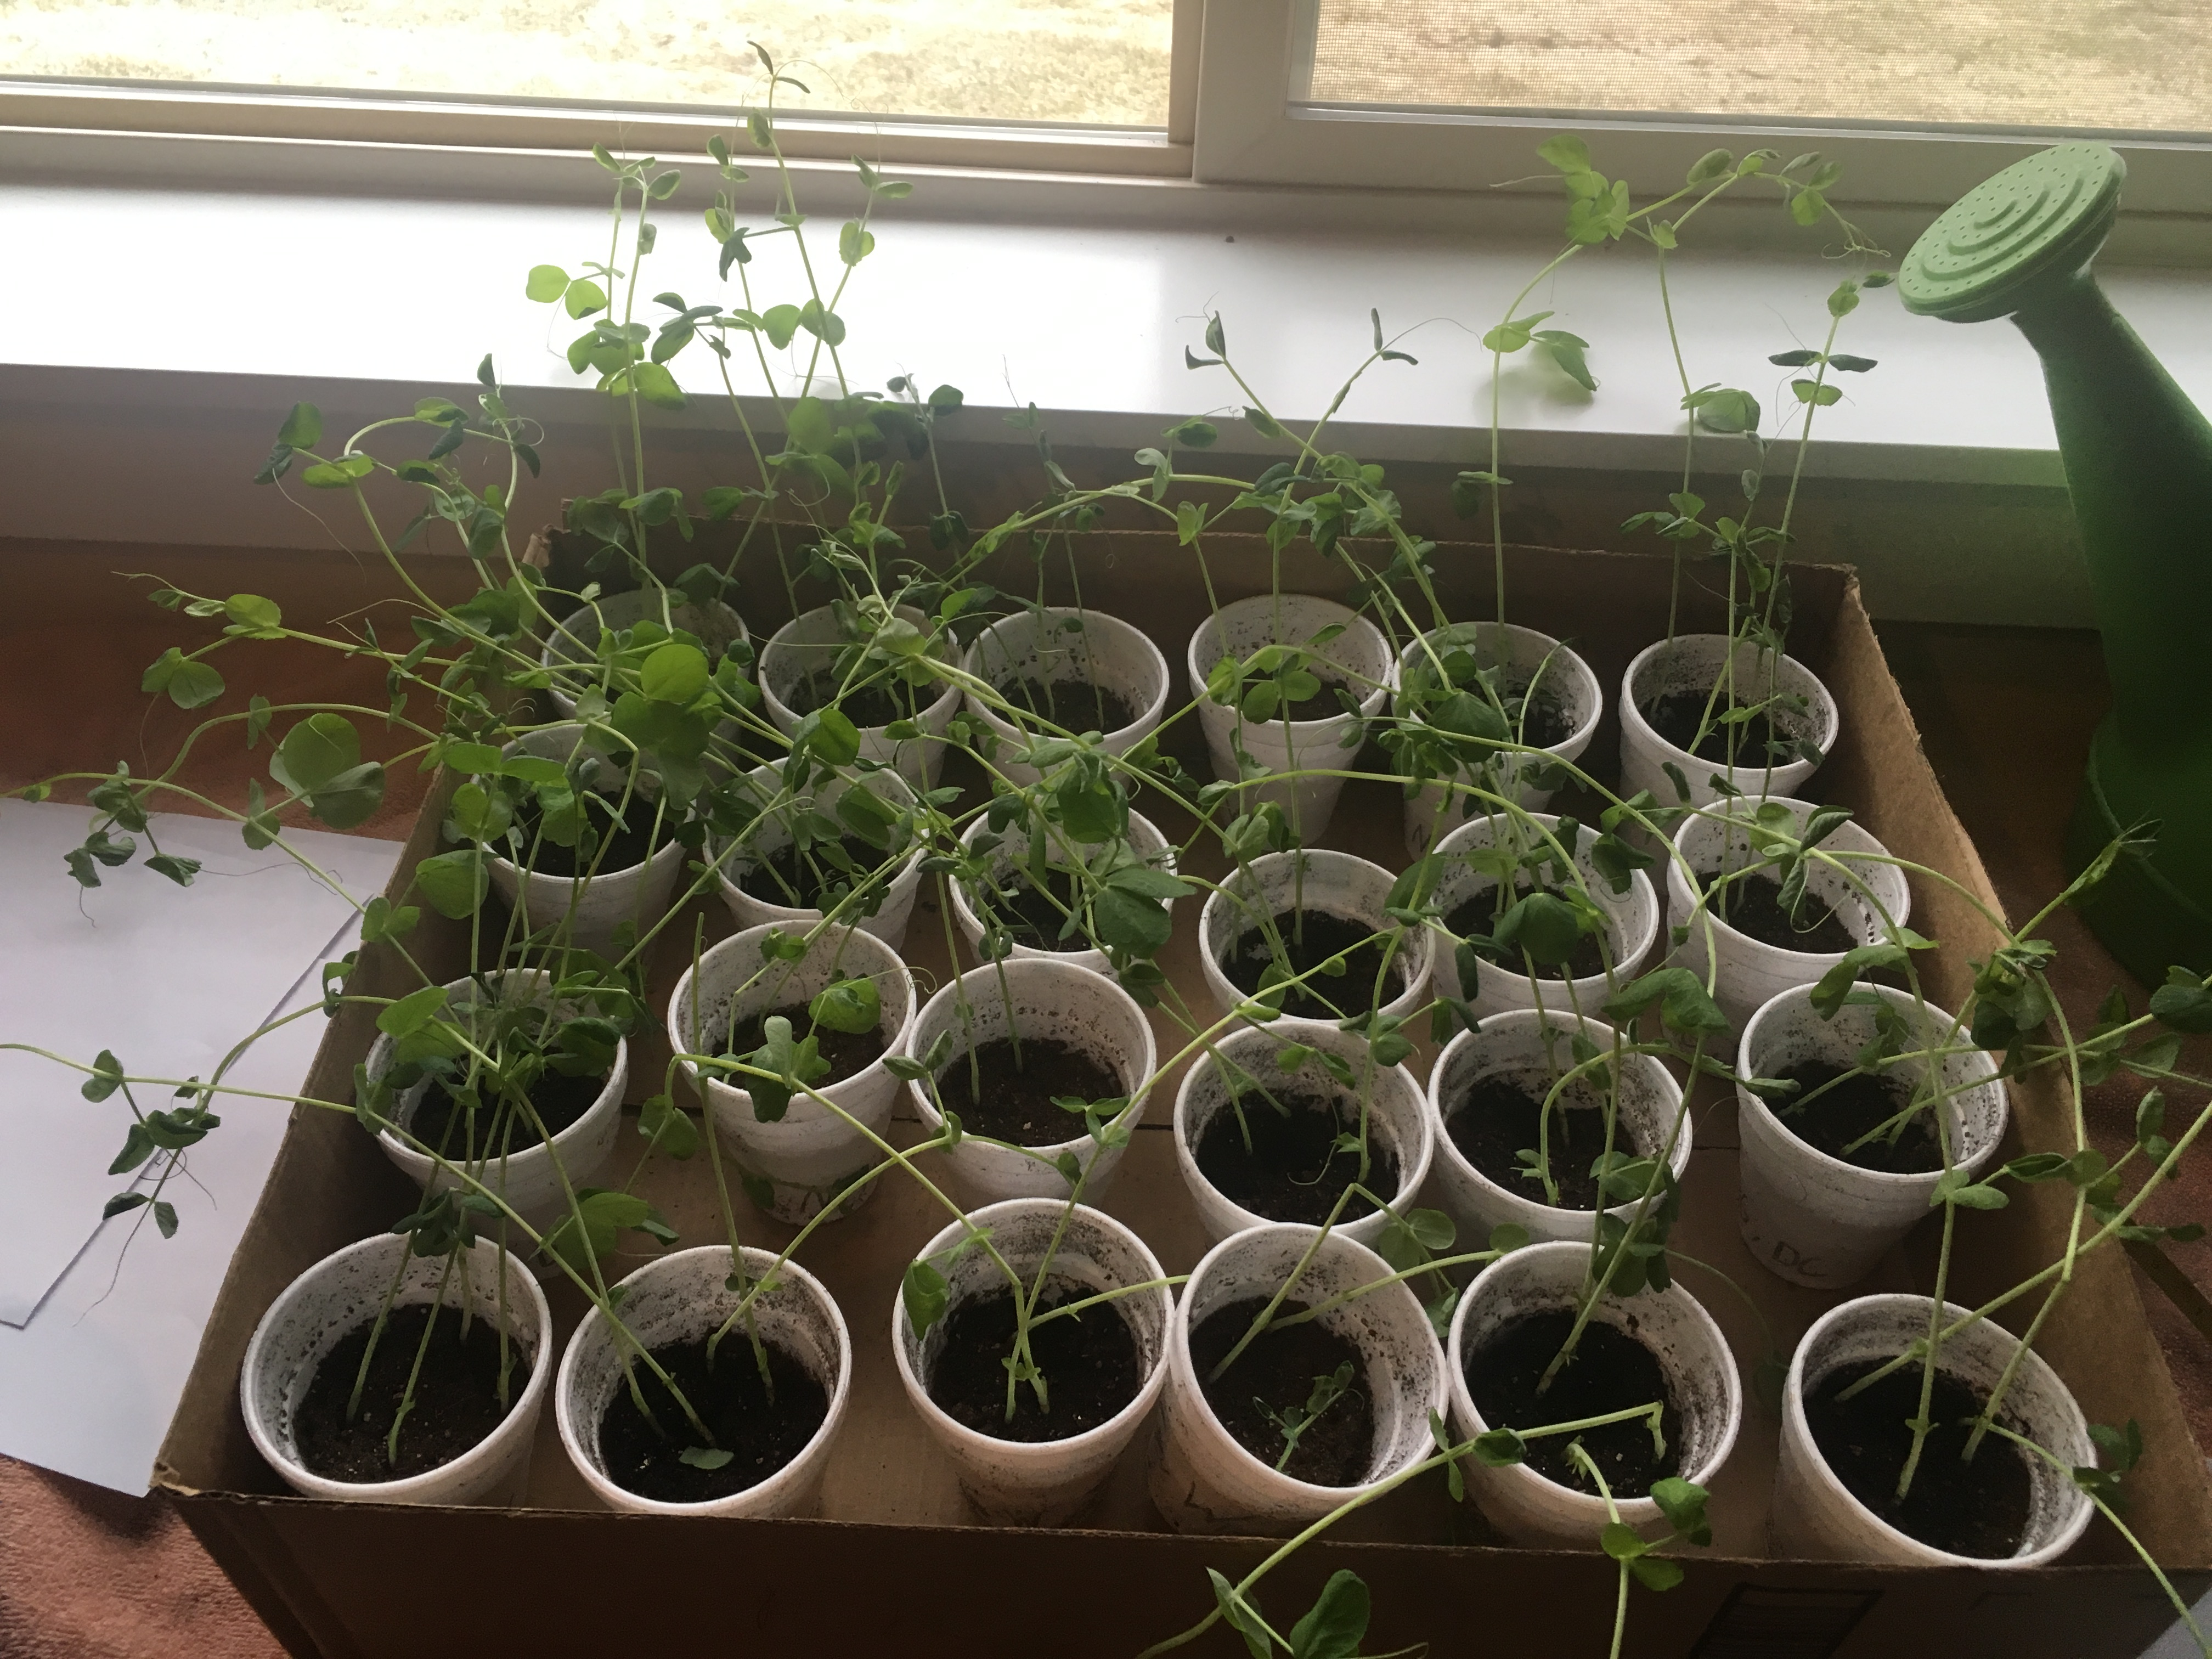
\includegraphics[width = 4cm]{figure/2weeks.JPG}
\end{figure}

Initial exploratory data analysis indicated fairly substantial differences in pea plant heights by treatment group. Overall, the mean plant height was 20.6 with a median height of 23 mm. This is slightly skewed left because of the 14 plants that did not germinate (these had a height of 0). When comparing by treatment combination, as is shown in the beanplot (Kampstra, 2008), we can compare distributions of plant heights by each treatment. The wide lines are the median heights for each group and the narrow lines refer to single observations. The median heights for the water-based groups appear to be lower than for either of the Diet-Coke based treatments. However, varaibilty in plant heights appears to be about the same for all groups. 

\begin{table}[ht]
\centering
\begin{tabular}{rrrrr}
  \hline
 & Min & Mean & Median & Max \\ 
  \hline
 & 0 & 20.6 & 23.0 & 40.0 \\ 
  
   \hline
\end{tabular}
\end{table}

\begin{knitrout}
\definecolor{shadecolor}{rgb}{0.969, 0.969, 0.969}\color{fgcolor}\begin{figure}
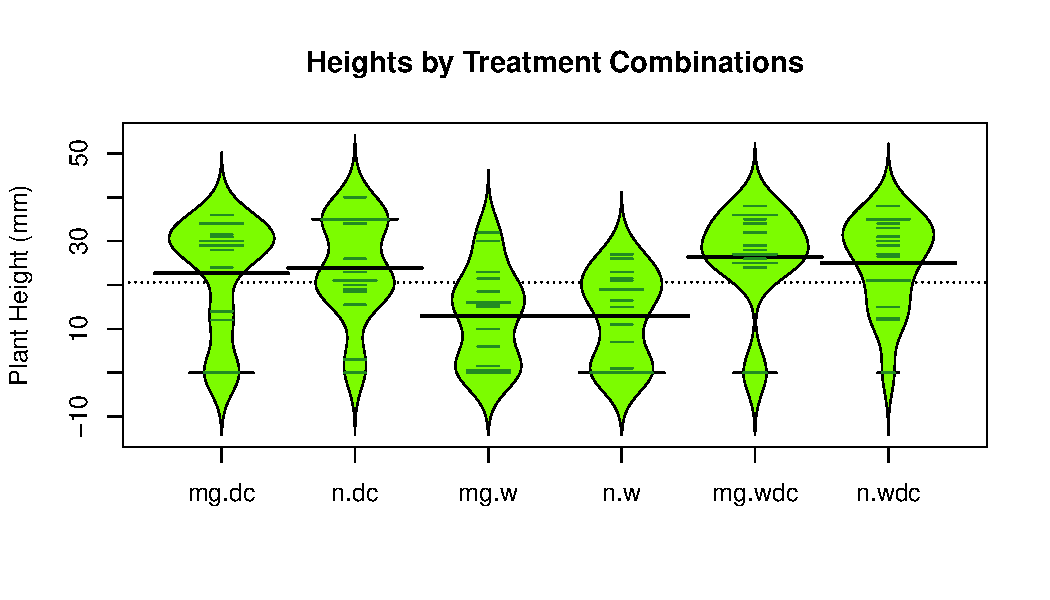
\includegraphics[width=\maxwidth]{figure/eda-1} \caption[Beanplot of heights by treatment group]{Beanplot of heights by treatment group.}\label{fig:eda}
\end{figure}


\end{knitrout}

There did not appear to be major differences in plant height by block, as shown in Figure X. This was expected as we did not anticipate major differences in plant conditions by block; however, we wanted the experiment to be designed in a way that was robust to such differences if they existed. 

\begin{knitrout}
\definecolor{shadecolor}{rgb}{0.969, 0.969, 0.969}\color{fgcolor}\begin{figure}
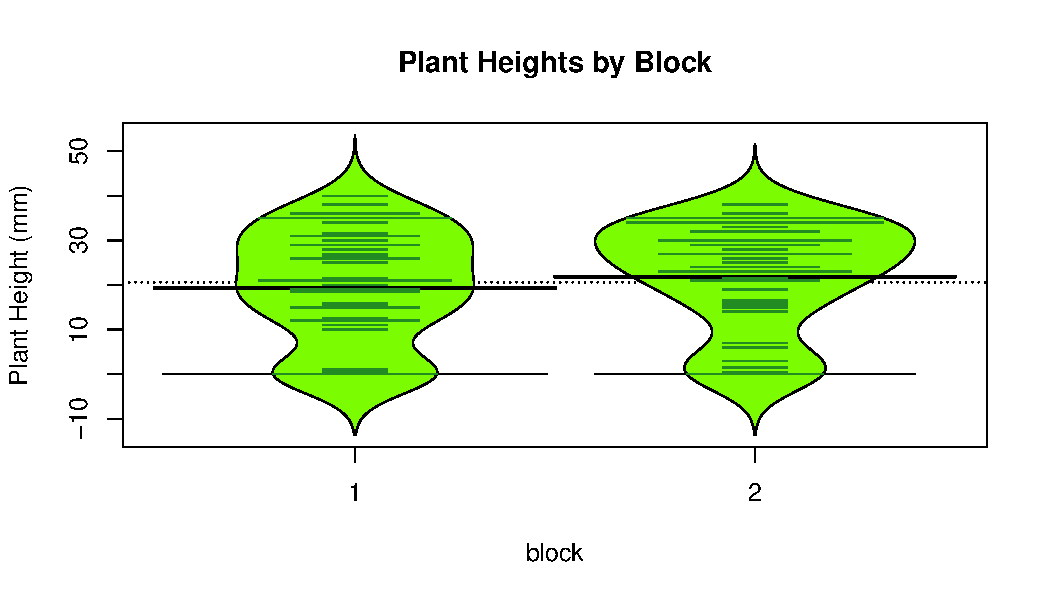
\includegraphics[width=\maxwidth]{figure/block_bean-1} \caption[Beanplot of heights by block]{Beanplot of heights by block}\label{fig:block_bean}
\end{figure}


\end{knitrout}


\subsection{Germination Rates}
Before we could do any statistical analysis of the pea plants, we had to determine that the treatment was not related to the germination probability for a given plant. Overall, 14 of the 82 (15 percent) of the pea plants failed to germinate. Figure X below shows the germination rates by each treament combination - there does not appear to be a large, systematic difference between the treatment combinations in terms of germination rates. 

\begin{knitrout}
\definecolor{shadecolor}{rgb}{0.969, 0.969, 0.969}\color{fgcolor}\begin{figure}
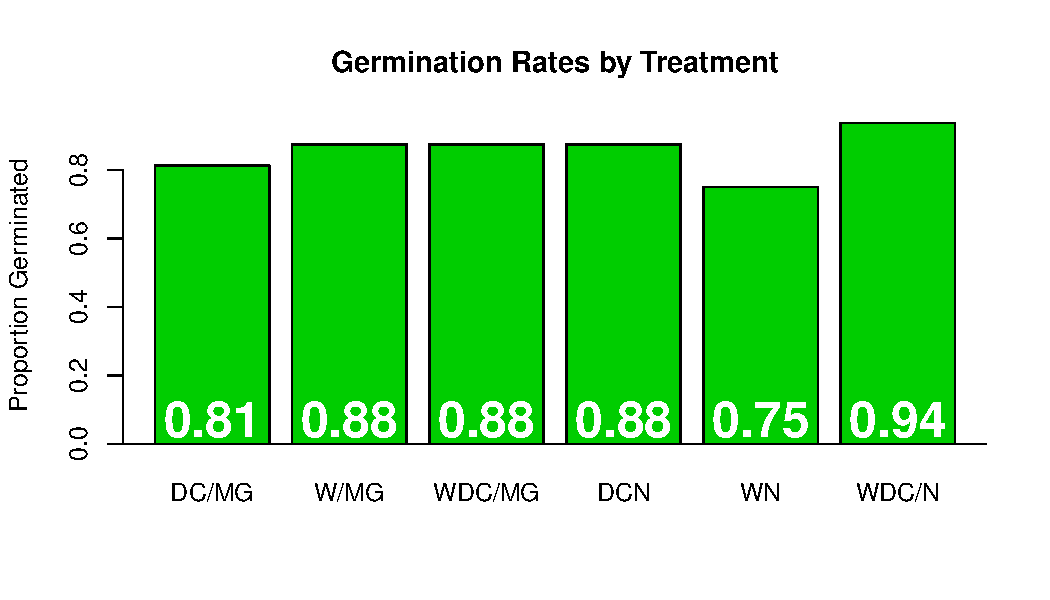
\includegraphics[width=\maxwidth]{figure/germination_rates-1} \caption[Germination rates by treatment group]{Germination rates by treatment group.}\label{fig:germination_rates}
\end{figure}


\end{knitrout}

A Chi-squared test of independence between the treatment groups and whether or not the plants germinated found no evidence that germination depended on treatment.  Since we did not find strong evidence supporting a relationship between germination probability and treatment, we treated the non-germinated plants as unobserved data in the analysis. 



\subsection{Regression Results}

All regressions and ANOVA were run using the lme4 package (Bates et al., 2015) and 'car' package (Fox, 2011). The results of the ANOVA are given below. Type II Sums of Squares were compared since the sample sizes within each treatment group were not even. The ANOVA table is given below for the fixed effects. The results are clear; the majority of variation in plant heights is driven by the watering treatment rather than by the presence of plant food.  The model finds strong evidence of height differences by Diet Coke treatment, based on a Wald chi-squared test with test statistic 31.42 on 2 degrees of freedom (with associated p-value < 0.0001). There was not strong evidence of a difference in plant heights by presence/absence of plant food nor was there evidence that the effect of watering substance differed depending on plant food treatment. 

% latex table generated in R 3.4.3 by xtable 1.8-2 package
% Fri Apr 20 15:40:25 2018
\begin{table}[ht]
\centering
\begin{tabular}{lrrr}
  \hline
 & Chisq & Df & Pr($>$Chisq) \\ 
  \hline
TrtCoke & 31.43 & 2 & 0.0000 \\ 
  PF & 0.13 & 1 & 0.7134 \\ 
  TrtCoke:PF & 1.40 & 2 & 0.4969 \\ 
   \hline
\end{tabular}
\end{table}
 

We also include effects plots (Fox, 2003) to describe the predicted means with associated uncertainty by treamtent group. The effects plots are included in Figure X. In the left panel, the predicted heights by watering treatment are given for plants that were treated with plant food. The right panel shows the predicted plant heights for those that were untreated by plant food. In both groups, the predicted heights for plants treated either with Diet Coke or diluted Diet Coke are at least 10 mm larger than for those treated with water. Even accounting for uncertainty in estimates, the confidence intervals for the Diet Coke treated plants are larger than for those that were treated with water only.  

\begin{knitrout}
\definecolor{shadecolor}{rgb}{0.969, 0.969, 0.969}\color{fgcolor}\begin{figure}
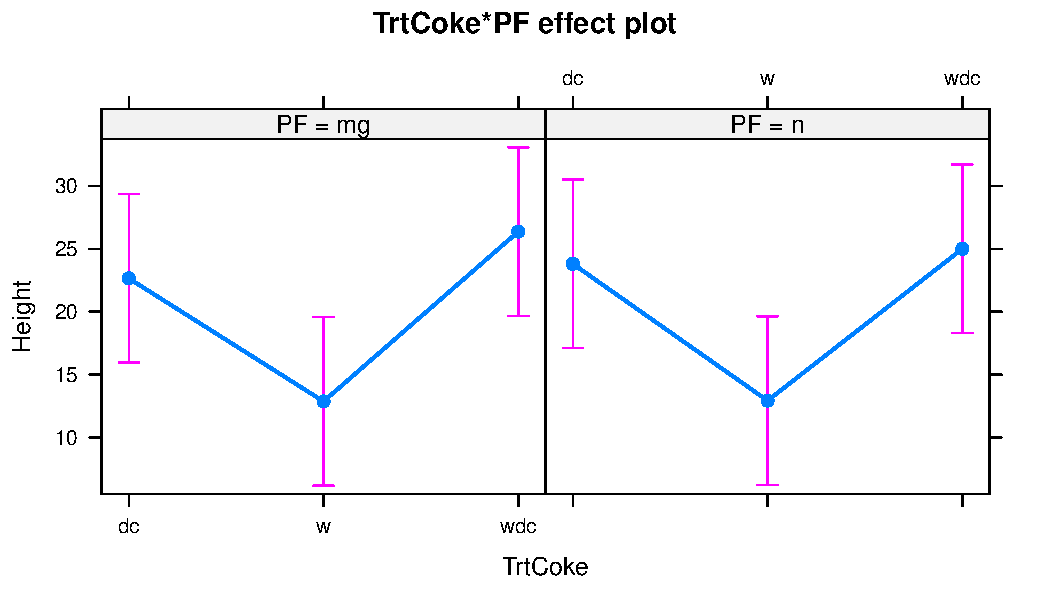
\includegraphics[width=\maxwidth]{figure/model_-1} \caption[Effects plot of the predicted means by treatment group]{Effects plot of the predicted means by treatment group}\label{fig:model }
\end{figure}


\end{knitrout}


\subsection{Tukey Pairwise Comparisons}

Tukey Honest Significant Differences were calculated for the pairwise comparisons between the treatment combinations. A compact letter display is given in Table X, with rankings by watering type averaged over the plant food factor. The rankings are such that rank 1 refers to the largest plant heights and rank 2 refers to the smallest plant heights.  The Tukey pairwise comparisons identify the Diet Coke and diluted Diet Coke treatments as having indisttinguishable mean plant heights, and the tap water treatment to be associated with smaller plant heights. 

% CLD table
\begin{table}[ht]
\centering
\begin{tabular}{lrrr}
  \hline
 & Diet Coke & Diluted Diet Coke & Water \\ 
  \hline
Ranking & 1 & 2 & 1 \\ 
  
   \hline
\end{tabular}
\end{table}


\section{Discussion}

\subsection{Conclusions}
This project illuminates some particularly interesting results. When we first started this analysis, we expected that the addition of Diet Coke to the watering regime of the pea plants would either harm or cause no benefit to the pea plants. This does not appear to be the case. Rather, the pea plants that were treated with either pure Diet Coke or Diet Coke dilution tended to grow at a more rapid rate than did those treated with just water. 

This may be reflective of the hardiness of alaskan pea plants in general. Or, it may be that the additional ingredients in the Diet Coke did not substantially harm the pea plants in the short term. 

\subsection{Limitations of the Study}

The alaska pea plants obtained from the study were purchased at Wal Mart and came from the Ferry Morse company. Because of proprietary differences in genetically-modified seeds, it is possible that these seeds differ from seeds sold by other companies. We do, however, assume that pea seeds within the company are randomly distributed. We randomly selected from the population of seeds that we purchased.  Treatments were randomly assigned to pea seeds. Therefore, we can make causal inference that among the population of Ferry Morse alaska pea plants, diet coke-based watering treatments caused  increased short-term growth relative to tap water-based watering regimes. 



\subsection{Future Work}
Pea plants are notoriously hardy. It may be that these plants were more resistant to the Diet Coke than other legumes or, for instance, annual flowers might be. Future research should consist of replicating this experiment with other types of plants.  Much of what motivated this study was the alarming amount of observational evidence that excessive consumption of Diet Coke has long-term health impacts on humans. Because pea plants make a poor proxy for human beings, eventually experiments like this should be conducted on people to compare health outcomes of Diet Coke drinkers to non-Diet Coke drinkers. The longitudinal studies that have already been done have laid the groundwork for identification of a relationship between health outcomes and soda consumption; however, to make causal inference between them, investigation via controlled experiments is sorely needed. 


\newpage
\section{Bibliography}

  Douglas Bates, Martin Maechler, Ben Bolker, Steve Walker (2015). Fitting Linear Mixed-Effects Models Using lme4. Journal of Statistical Software, 67(1), 1-48. doi:10.18637/jss.v067.i01.
~ \\ 

John Fox and Sanford Weisberg (2011). An {R} Companion to Applied Regression, Second Edition. Thousand Oaks CA: Sage. URL:  http://socserv.socsci.mcmaster.ca/jfox/Books/Companion
~\\

Peter Kampstra (2008). Beanplot: A Boxplot Alternative for Visual Comparison of Distributions. Journal of Statistical Software, Code Snippets 28(1). 1-9. URL http://www.jstatsoft.org/v28/c01/.
~ \\ 


Levitt, Steven D. (2007) \textit{Diet Coke is 99 percent water (And That Is Now a Good Thing) }. Freakonomics. http://freakonomics.com/2007/08/20/diet-coke-is-99-water-and-that-is-now-a-good-thing/
~\\

Matthew P. Pase, Jayandra J. Himali, Alexa S. Beiser, Hugo J. Aparicio, Claudia L. Satizabal, Ramachandran S. Vasan, Sudha Seshadri and Paul F. Jacques. 
\textit{Sugar- and Artificially Sweetened Beverages and the Risks of Incident Stroke and Dementia.} 
Stroke. 2017;48:1139-1146, April 24, 2017
~\\

Nielsen Company, The. 2016. FMCG and Retail Insights.
~\\  

Roland, M. (2013). "The Effects of Vitamin Water on Pea Plant Growth". Retrieved from https://prezi.com/domu2sdet-w5/the-effects-of-vitamin-water-on-pea-plant-growth/ \\ 
~ \\ 

Slutzky, B., Douglas, C., Hofman, S., Greenstein, E., & Reilly, A. (2003). "Pea Plant Experiments." Retrieved from http://web.mph.net/academic/science/mvural/Life%20Science/Pea%20Plant%20Experiments.htm 
~ \\ 

Singleton, Bonnie. (2018). Alaskan Pea Plant Development. Home Guides | SF Gate. Retrieved from http://homeguides.sfgate.com/alaskan-pea-plant-development-56566.html
~\\

Tayeh, N., G. Aubert, M.L. Pilet-Nayel, I. Lejeune-Henaut, T.D. Warkentin and J.
Burstin. 2015. Genomic Tools in Pea Breeding Programs: Status and Perspectives.
Frontiers in Plant Science 6: 13. doi:10.3389/fpls.2015.01037.
~\\  

Veldhuizen, Maria Geraldine et al.
Current Biology , Volume 27 , Issue 16 , 2476 - 2485.e6
~\\


\end{document}
